\section{Type Inference}
\label{sec:type-inference}

\name's region type system imposes a heavy annotation burden, and the
cost of manually annotating C\# standard libraries with region types
is prohibitive. We now present our region type inference algorithm
that completely eliminates the need to write region type annotations,
except on some higher-order functions. Formally, the type inference
algorithm is an elaboration function from programs in $\absof{\FB}$
(i.e., \FB without region types, but with \C{letregion} and \C{open}
expressions, similar to the language introduced in
\S~\ref{sec:overview}) to programs in \FB. The key aspects of this
elaboration are described below.

% We formalize region type inference as an elaboration function from
% programs in $\absof{\FB}$ (i.e., region annotation-erased \FB) to
% programs in \FB.  The elaboration proceeds in four steps. In the first
% step we make use of the observation that region types are
% \emph{refinements} of FGJ types with region annotations and
% constraints over such region annotations, and compute polymorphic
% region type templates for methods and classes from their FGJ types.
% The templates contain region variables ($\rho$) to denote unknown
% region annotations, and predicate variables ($\varphi$) to denote
% unknown constraints over such region annotations. Free region
% variables are generalized in types (hence, polymorphic). Second, we
% elaborate expressions by introducing region variables to denote
% unknown region arguments in \C{new} expressions, method calls and
% function applications. While elaborating expressions, we make use of
% the computed region type templates to build a system of constraints
% that capture well-formedness requirements and subtyping relationships
% between type templates that must hold (as per the static semantics in
% Fig.~\ref{fb-staticsem}) for the elaboration to be valid.  Third, we
% lift expression elaboration and constraint generation to methods and
% classes. Finally, we solve the constraints to compute solutions to
% region ($\rho$) and predicate ($\varphi$) variables.
%
% Due to the presence of region-polymorphic
% recursion in \FB, constraints generated by the algorithm can be
% circular. More precisely, constraints generated can assume the form
% $\varphi \Leftrightarrow \phi \wedge F(\varphi)$, where $F$ is a
% non-idempotent substitution function for region variables in
% $\varphi$. In the constraint solving phase, the algorithm then relies
% on a fixpoint constraint solving algorithm called \csolvestar to solve
% the constraints and determine assignments for unknown region and
% predicate variables.

\subsection{Region Type Templates}
\label{sec:fb-templatization}

Region type templates are FGJ types extended with fresh region
variables ($\rho$) and predicate variables ($\varphi$) to denote
unknown region annotations and region constraints, respectively. For
instance, if a variable $x$ has type $\ObjZ$ in FGJ, its region type
template is of form $\ObjZ\inang{\rho_0}$, where $\rho_0$ is a fresh
region variable. FGJ type $\RgnZ\inang{T}$ is special; it is always
templatized as $\RgnZ{\inang{T}}\inang{\toprgn}$. Given the
region-annotated definition of \C{Pair} class from
\S\ref{sec:fb-syntax} a region type template for a method with FGJ
type $\C{Pair}\inang{\C{A},\C{B}} \rightarrow \C{A}$ is \footnote{In
our exposition, we assume that classes $\C{A}$ and $\C{B}$ are trivial
subclasses of $\ObjZ$ with no fields/methods. Like $\ObjZ$, they
accept one region parameter - the allocation region of their
objects.}\footnote{We abuse arrow notation to also represent types of
methods, but unlike function types, there is no allocation region
annotation atop the arrow.}
$\inang{\rhoalloc_0,\rho_{1-4} \,|\, \varphi_0}
\C{Pair}\inang{\C{A},\C{B}} \inang{\rho_{1-3}} \rightarrow
\C{A}\inang{\rho_4}$, where $\rhoalloc_0$ and $\rho_{1-3}$ are fresh
region variables, and $\varphi_0$ is a fresh predicate variable
denoting unknown constraints over $\rhoalloc_0$ and $\rho_{1-3}$.
Region type template of a type variable $\C{a}$ is $\C{a}@\rho$, where
$\rho$ is fresh. For a class, a template is computed based on the 
type templates of its fields, constructors and methods. Additional
region and predicate variables are added as necessary. Following template 
of the \C{Pair} class illustrates this point:
% For a class, a template is computed in two steps. In
% the first step, we templatize the types of all its fields, constructor
% arguments, and arguments and return values of all its methods, along
% with the type of its superclass. In the second step, we generalize all
% the free region variables occuring in the templates computed in the
% first step as region parameters of the class. Finally, we add a fresh
% allocation region parameter ($\rhoalloc$) to the list of parameters,
% and introduce a new predicate variable ($\varphi$) to denote unknown
% constraints on region parameters. For example, consider the standard
% FGJ definition of $\C{Pair}\inang{\C{a},\C{b}}$ class, where $\C{a}$
% and $\C{b}$ are the types of $\C{fst}$ and $\C{snd}$ fields,
% respectively. It can be templatized as following :
\vspace*{-0.1in}
\begin{center}
\begin{codejava}
class Pair$\inang{a\extends\ObjZ, b\extends\ObjZ}$
          $\inang{\rhoalloc_0,\rho_{0-4}\,|\,\varphi_0} \extends \ObjZ\inang{\rho_4}$ {
  $a@\rho_0$ fst; $b@\rho_1$ snd;
  Pair($a@\rho_2$ fst, $b@\rho_3$ snd) { 
    super(); this.fst=fst; this.snd=snd; 
  }
  a@$\rho_5$ getFst$\inang{\rhoalloc_1,\rho_5\,|\,\varphi_1}$() { return this.fst; }
}
\end{codejava}
\end{center}
\vspace*{-0.1in}
% \footnote{In reality, the generalized region variables only come
% from the type templates of class's fields and superclass. Method
% types do not contain any free region variables.}
% The template elides $\C{Pair}$'s methods, whose region type
% templates contain no free variables. Among the region parameters of
% the class template, $\rho_{0-4}$ are obtained by generalizing free
% region variables in the types of its class's fields, constructor
% arguments, and its superclass type.  The remaining parameter
% ($\rhoalloc_0$) is a fresh region variable denoting the allocation
% region argument. Fresh predicate variable $\varphi_0$ denotes
% unknown constraints over $\rhoalloc_0$ and $\rho_{0-4}$ that need to
% hold for template to be a well-formed region-annotated class
% definition in $\FB$. 
%
% The type template for a recursively defined class is computed in two
% steps. First, all recursive occurances of the class among the types of
% its fields are ignored and the class is templatized as if it is a
% non-recursive class. Next, all the recursive occurances are
% templatized with respect to the class template computed in the first
% step, such that their region annotations are \emph{exactly} same as
% the region parameters of the class. Applying this technique on a
% recursively defined $\C{LinkedListNode}\inang{\C{a}}$ class, for
% example, results in a template that uses same region variable to
% denote allocation regions of the current node, and the node that the
% current node refers to. 
%
% For example, consider a generic $\C{ListNode}\inang{\C{a}}$ class
% containing two fields: $\C{data}$ of type $\C{a}$ and $\C{next}$ of
% type $\C{ListNode}\inang{\C{a}}$.  where $\C{a}$ is the type of the
% data stored in the linked list node.  To templatize the
% $\C{ListNode}\inang{a}$ class, we first ignore its recursive
% occurance in the type of $\C{next}$ field, and templatize the type
% $\C{a}$ of $\C{data}$ field as $\C{a}@\rho_0$. Based on this type
% template of $\C{data}$ field, we compute the class's template as
% following: \begin{center} $\C{ListNode}\inang{\C{a}\extends\ObjZ}
% \inang{\rhoalloc_0,\rho_0\,|\,\varphi_0} \extends \ObjZ \{...\}$
% \end{center} Next, we trivially templatize the type of $\C{next}$
% field in the body of the class as
% $\C{ListNode}\inang{\C{a}}\inang{\rhoalloc_0,\rho_0}$.  The
% resulting class represents a linked list with spine in the region
% $\rhoalloc_0$ and data objects in the region $\rho_0$.
% Observe that our strategy of trivially templatizing the recursive
% occurances of a class type in its definition ensures that no new
% region variables are introduced.
The type template for for a recursively defined class is computed in
two steps. First, a template is computed by ignoring the recursive
occurrences. Next, all the recursive occurrences are templatized based
on the template computed in first step.  This approach can be extended
to mutually recursive definitions in a straightforward manner. Using
the techniques outlined above, we compute region type templates for
all classes bound in the class table of the $\absof{\FB}$ program
before we proceed to elaborate expressions.

%\begin{figure}

\begin{codeml}
$\elabExpr(CT, \A, \ralloc, \env, e)$ = 
  match $e$ with
  | $\C{new} \fgjN(\bar{e})$ $\longrightarrow$ 
    let $\fbN$ = $\templateTy(\fgjN)$ in
    let $C_1$ = $\typeOk({\A},{\fbN})$ in
    let $C_2$ = match $\fgjN$ with $\RgnZ\inang{T}$ $\longrightarrow$ $\top$
          | _ $\longrightarrow$ $\{\isvalid{\A.\phicx}{\allocRgn(\fbN)=\ralloc}\}$ in
    let ($\_:\taubar$) = $\fields(\fbN)$
    let $(\bar{e'}:\bar{\tau'}, C_3)$ = $\elabExpr(\A,\ralloc,\env,\bar{e})$ in
    let $C_4$ = $\subtypeOk({\A},{\bar{\tau'}},{\taubar})$ in
      ($\C{new} \fbN(\bar{e'}) : \fbN$,$\bigcup_{i=1}^4 C_i$)
  | $e_a(\bar{e})$ $\longrightarrow$ 
    let ($e_a':\inang{\rhoalloc\rhobar\,|\,\phi}\taubar \xrightarrow{\rgn} \tau$,$C_1$) = 
                $\elabExpr(\A,\ralloc,\env,e_a)$ in
    let $\bar{\rho'}$ = $\bar{\fresh_\rho()}$ in
    let $C_2$ = $\{\bar{\rho'} \in \A.\rhoenv\}$ in
    let $\substFn$ = $[\bar{\rho'}/\rhobar][\ralloc/\rhoalloc]$ in
    let $C_3$ = $\{\isvalid{\A.\phicx}{\substFn(\phi)}\}$ in
%*   %let $(C_3,C_4)$ = $(\typeOk(\substFn(\taubar)), \typeOk(\substFn(\tau)))$ in 
*)   let $(\bar{e'}:\bar{\tau'}, C_4)$ = $\elabExpr(\A,\ralloc,\env,\bar{e})$ in
    let $C_5$ = $\subtypeOk({\A},{\bar{\tau'}},{\bar{\substFn(\tau)}})$ in
      ($e_a'\inang{\ralloc\bar{\rho'}}(\bar{e'}):\substFn(\tau)$,$\bigcup_{i=1}^5 C_i$)
  | $\letregion{\rgn}{e_a}$ $\longrightarrow$
    let $\rgn'$ = $\fresh_{\rgn}()$ in 
    let $(\rhoenv,\aenv,\phicx)$ = $\A$ in
    let $\A'$ = ($\rhoenv \cup \{\rgn'\}, \aenv, \phicx \conj (\rhoenv \outlives \rgn')$) in
    let ($e_a':\tau$,$C_1$) = $\elabExpr(\A',\rgn',\env,[\rgn'/\rgn]e_a)$ in
      ($\letregion{\rgn'}{e_a'}:\tau$,$C_1$)
  | $\open{e_a}{\rgn}{y}{e_b}$ $\longrightarrow$ 
    let ($e_a':\RgnZ\inang{T}\inang{\rho}$,$C_1$) = 
                $\elabExpr(\A,\ralloc,\env,e_a)$ in
    let $\rgn'$ = $\fresh_{\rgn}()$ in 
    let $(\rhoenv,\aenv,\phicx)$ = $\A$ in
    let ($\A'$,$\env'$) = ($(\rhoenv \cup \{\rgn'\},\aenv,\phicx)$,$\env[y\mapsto T@\rgn']$) in
    let ($e_b':\tau$,$C_2$) = $\elabExpr(\A',\rgn',\env',[\rgn'/\rgn]e_a)$ in
      ($\open{e_a'}{\rgn'}{y}{e_b'} : \tau$, $C_1 \cup C_2$)
  | _ $\longrightarrow$ ...
\end{codeml}

\caption{Constraint generation for expressions in $\absof{\FB}$}
\label{fig:fb-elabexpr}
\end{figure}

%\newcommand{\hdOf}[2]{\C{class}\; #1\angAlpha\inang{\rhoalloc\rhobar \,|\, #2} \extends \fbN}
\begin{figure}

\begin{codeml}
$\elabMeth(CT, B, \tau \; m\inang{\rhoalloc_m\rhobarm \,|\, \varphi_m} (\taubar \; \xbar)\{\C{return} e;\})$ = 
  let $\hdOf{B}{\varphi}\{\bar{\tau^f}\,\xbar;\;k\;\bar{d}\}$ = $CT(B)$ in
  let ($\rhoenv$,$\aenv$,$\phicx$) as $\A$ = 
            $(\{\rhoalloc,\rhobar,\rhoalloc_m,\rhobarm\},\bar{\tyvar} \extends \bar{\fgjN},\varphi \conj \varphi_m)$ in
  let $C_1$ = $\{\tywf{\rhoenv}{\varphi_m}\}$ in
  let $\env$ = $\cdot[\thisZ \mapsto B\inang{\bar{\tyvar}}\inang{\rhoalloc\rhobar}][\xbar \mapsto \taubar]$ in
  let ($e':\tau'$,$C_2$) = $\elabExpr (\A,\rhoalloc_m,\env,e)$ in
  let $C_3$ = $\subtypeOk({\A},{\tau'},{\tau})$ in
    ($\tau \; m\inang{\rhoalloc_m\rhobarm \,|\, \varphi_m} (\taubar \;
    \xbar)\{\C{return} e';\}$, $C_1 \cup C_2 \cup C_3$)
\end{codeml}

\begin{codeml}
$\elabClass(CT,B)$ = 
  let $\hdOf{B}{\varphi}\{\bar{\tau^f}\,\xbar;\;k\;\bar{d}\}$ = $CT(B)$ in
  let ($\rhoenv$,$\aenv$,$\phicx$) as $\A$ = $(\{\rhoalloc,\rhobar\},\bar{\tyvar} \extends \bar{\fgjN},\varphi)$ in
  let $C_1$ = $\tywf{\rhoenv}{\varphi}$ in
  let ($C_2$,$C_3$) = ($\typeOk({\A},{\fbN})$,$\typeOk({\A},{\bar{\tau^f}})$) in
  let $C_4$ = $\{\isvalid{\phicx}{\allocRgn(\bar{\tau^f}) \outlives \rhoalloc \conj \allocRgn(\fbN) = \rhoalloc}\}$ in
  let ($k'$,$C_5$) = $\elabCons(B,k)$ in
  let ($\bar{d'}$,$C_6$) = $\elabMeth(B,\bar{d})$ in
    ($\hdOf{B}{\varphi}\{\bar{\tau^f}\,\xbar;\;k'\;\bar{d'}\}$, $\bigcup_{i=1}^6 C_i$)
\end{codeml}
%
% \begin{codeml}
% $\elabClassTable(CT)$ = 
%   let ($CT'$,$C$) = (ref $\cdot$, ref $\emptyset$) in
%   let _ = foreach $B \in dom(CT)$ do
%             let ($D_B$,$C_B$) = $\elabClass(CT,B)$ in
%               $CT'$ := $CT'[B \mapsto D_B]$;
%               $C$ := $C \cup C_B$
%            done in
%   let ($\substFn_\rho$,$\substFn_\varphi$) = $\solve(C)$ in
%     $\substFn_\varphi(\substFn_\rho(CT')) $
%       
% \end{codeml}

\caption{Method, class and class table elaboration}
\label{fig:fb-elabmeth}
\end{figure}


\subsection{Elaboration and Constraint Generation}

Elaborating $\absof{\FB}$ expressions to $\FB$ expressions involves
(a). replacing core types occurring in expressions with fresh region
type templates, and (b). explicitly instantiating region parameters
with fresh region variables in method calls and function applications.
This elaboration is performed with respect to the polymorphic type
templates of classes and methods computed as per
\S\ref{sec:fb-templatization}. Our expression elaboration
function\footnote{Supplement contains the pseudocode for all the
elaboration functions.} traverses expressions in a syntax-directed
manner of a type checker, introducing fresh region type templates for
unknown region types, while generating constraints over region and
predicate variables. The precise nature of generated constraints is
explained in \S\ref{sec:constraints}, but in summary, they
capture the relationships between the type templates of various
subexpressions and their well-formedness.

% Function $\elabExpr$, shown in Fig.~\ref{fig:fb-elabexpr}, performs
% this elaboration for a subset of expressions in $\absof{\FB}$
% %, whose corresponding $\FB$ expressions have been ascribed static
% %semantics in Fig.~\ref{fig:fb-staticsem}. 
% $\elabExpr$ is defined under the same context as the expression typing
% judgment in Fig.~\ref{fig:fb-staticsem} with symbols $\A$,$\ralloc$,
% and $\env$ retaining their meaning. The function traverses expressions
% in a syntax-directed manner of a type checker, introducing fresh
% region type templates for unknown region types, while generating
% constraints over region and predicate variables. The precise nature of
% generated constraints is explained in \S\ref{sec:fb-constraintsem},
% but in summary, they capture the relationships between the type
% templates of various subexpressions and their well-formedness. Note
% that $\elabExpr$ returns the region type template of the
% subexpression, which is used to generate constraints for the
% expression. Functions $\typeOk$ and $\subtypeOk$ (definitions not
% shown) used by $\elabExpr$ implement type well-formedness and subtype
% judgments from Fig.~\ref{fig:fb-staticsem}, respectively.

Expression elaboration can be trivially lifted to the level of a
method, and method elaboration to the level of a class, while
accumulating constraints. Besides such constraints, elaboration
functions for methods and classes also generate new constraints by
checking well-formedness and subtype relationships among the types of
their constituents. For instance, method elaboration generates a new
constraint that captures the requirement that, under the guarantees
provided by the context, the region type of a method body must be a
subtype\footnote{Subtyping is type equality in \FB. In \name,
subtyping between region types is a straightforward extension of
subtyping between core types.} of method's return type.  Likewise, the
elaboration function for a class generates a fresh constraint that
captures a couple of safety conditions: first, the allocation regions
of objects referred by the instance variables should outlive the
allocation region of the instance itself, and second, the allocation
regions of a class type and its superclass type must be the same.

Elaborating a class table ($CT$) entails elaborating every class
definition in $CT$, while collecting constraints. The constraints thus
collected are finally solved to obtain assignments for free region and
predicate variables introduced during templatization and elaboration
stages. The solutions are applied to the class table (and to the
artifacts that make up the class table, recursively) to compute a
class table that maps classes to their fully region-annotated
definitions in $\FB$.

% \subsection{Method and Class Elaboration}

% Elaborating a method involves performingexpression elaboration over
% its body, while collecting constraints. Method elaboration can be
% lifted to the level of classes


% Functions $\elabMeth$ and $\elabClass$ shown in
% Fig.~\ref{fig:fb-elabmeth} lift expression elaboration to method and
% class definitions, respectively. Both functions first build a context
% ($\A$) containing a set ($ \rhoenv$) of regions that are currently
% live, a map ($\aenv$) mapping type variables to their bounds, and a
% constraint formula ($\phicx$) capturing constraints over live region
% variables. We use predicate variables ($\varphi$ and $\varphi_m$) to
% capture constraints over variables in $\rhoenv$ denoting the fact that
% such constraints are yet to be inferred. Both elaboration functions
% generate new constraints by checking well-formedness and subtype
% relationships among types of their constituents. A fresh constraint
% ($C_4$) generated by $\elabClass$ captures a couple of safety
% conditions: first, the allocation regions of objects referred by the
% instance variables should outlive the allocation region of the
% instance itself, and second, the allocation regions of a class type
% and its superclass type must be the same.

% Function $\elabMeth$ elaborates a method definition of class $B$. It
% calls $\elabExpr$ with the context $\A$, its allocation context
% parameter ($\rhoallocm$), and a type environment ($\env$) that
% contains region type bindings for all the arguments of the method,
% including the implicit $\C{this}$ argument. The region type template
% returned by $\elabExpr$ for the method body is checked against its
% expected type (derived from the type template of the method)
% generating more constraints. The function then returns the elaborated
% method definition and the set of constraints.

% $\elabClass$ elaborates the definition of a class $B$. It relies on
% $\elabCons$ (not shown) and $\elabMeth$ functions to elaborate $B$'s
% constructor ($k$) and method definitions ($\bar{d}$), respectively. To
% the set of constraints returned by these functions, $\elabClass$ adds
% constraints generated by checking the well-formedness of the type
% templates of its superclass and fields, and also a new constraint
% capturing a couple of safety conditions: first, the allocation regions
% of objects referred by the instance variables should outlive the
% allocation region of the instance itself, and second, the allocation
% regions of a class type and its superclass type must be the same.

% Function $\elabClassTable$ (not shown) elaborates
% every definition in the class table $CT$, while accumulating
% constraints. The constraints are finally solved for free region and
% predicate variables introduced during templatization and elaboration
% stages. The solutions are applied to the class table (and to the
% artifacts that make up the class table, recursively) to compute a
% class table that maps classes to their fully region-annotated
% definitions in $\FB$.

% Note that if the original program in $\absof{\FB}$ contains unsafe
% references, for example, a reference from a transferable region to a
% stack regions, then the constraints generated during the elaboration
% are not satisfiable. In such case, $\solve$ fails to solve
% constraints, causing the program to be rejected.

\subsection{Constraints}
\label{sec:constraints}

Three kinds of constraints are generated during elaboration:
\begin{itemize}
\item Well-formedness constraints of form $\rho \in \rhoenv$,
restricting the domain of unification for a region variable ($\rho$)
to the set ($\rhoenv$) of regions in scope,
\item Well-formedness constraints of form
$\tywf{\rhoenv}{\varphi}$, restricting the domain of a predicate
variable ($\varphi$) to the set of all possible constraint formulas
over region variables ($\rhoenv$) in scope, and
\item Validity constraints of form $\isvalid{\phicx}{\phi}$, where
$\phicx$ and $\phi$ are region constraints (Fig.~\ref{fig:fb-syntax})
extended with predicate variables and \emph{pending
substitutions}\footnote{we borrowed this terminology
from~\cite{ltpldi08}}:
\begin{smathpar}
\begin{array}{lcl}
\phicx,\phi & \coloneqq & true \ALT \rho \outlives \rho \ALT \rho = \rho 
    \ALT F(\varphi) \ALT \phi \conj \phi\\
F & \coloneqq & \cdot \ALT [\rho/\rho]F \\
\end{array}
\end{smathpar}
\end{itemize}
A pending substitution ($F$) is a substitution function over region
variables/identifiers. They represent the substitutions that need to
be carried out when a predicate variable ($\varphi$) is replaced by a
concrete formula in a validity constraint. For instance, in the
validity constraint $\isvalid{\rgn_1 \outlives
\rgn_2}{[\rgn_1/\rho_1][\rgn_2/\rho_2]\varphi}$, pending substitution
is $[\rgn_1/\rho_1][\rgn_2/\rho_2]$. Any concrete formula (call it
$\phisol$) over variables $\rho_1$ and $\rho_2$ is a solution to
$\varphi$ if and only the formula obtained by substituting $\rgn_1$
and $\rgn_2$ for $\rho_1$ and $\rho_2$ (resp.) in $\phisol$ is
deducible from $\rgn_1 \outlives \rgn_2$.
% Validity constraints primarily result from checking if a region type
% template of form $B\inang{\tbar}\inang{\rhoalloc,\rhobar}$ is
% well-formed (i.e., $\typeOk$). The corresponding well-formedness rule
% (Fig.~\ref{fig:fb-staticsem}) requires that the instantiation of $B$'s
% formal region parameters with actual region arguments satisfy its
% precondition, where actuals are subsituted for formals. Since $B$'s
% precondition could be unknown, the requirement results in a in a
% validity constraint with predicate variables and pending
% substitutions. Other sources of validity constraints are calls to
% region-polymorphic methods, where similar situation arises. 
% In general, validity constraints generated by our algorithm assume one
% of the following two forms:
% \begin{center}
% \( \isvalid{\phictxt \conj \bigwedge_{i}\varphi_i}
%            {\phicstr} \qquad
%    \isvalid{\phictxt \conj \bigwedge_{i}\varphi_i}
%            {F_j(\varphi_j)}
% \)
% \end{center}
% Where $\varphi_i$'s denote the unknown preconditions of the class and
% the method under elaboration. If the constraint is generated while
% checking the well-formedness of a type or elaborating an expression,
% then $\varphi_j$'s denote the unknown preconditions of classes and
% methods that were used in that type or expression. Each use of a
% (region-polymorphic) class or a method has to instantiate region
% parameters, resulting in pending substitutions ($F_j$). Formulas
% $\phictxt$ and $\phicstr$ are concrete, i.e., free of predicate
% variables and pending substitutions. While $\phictxt$ captures
% relationships that are \emph{known} to hold between concrete region
% identifiers (i.e., $\rgn$'s) when the constraint was generated,
% $\phicstr$ captures relationships that are \emph{required} to hold
% among region varibles (i.e., $\rho$'s), or relationships between
% region variables and identifiers. Each region variable occuring in
% $\phicstr$ has an associated well-formedness constraint, which
% specifies its unification domain. The unification domain of a
% constraint is the union of unification domains of all region variables
% occuring in the constraint.

\paragraph{Constraints Example 1} Consider the $\C{Pair}$ class
template from \S\ref{sec:fb-templatization}. Following constraints are
generated during its elaboration (Constrains are identified with
$\mathbf{c_i}$'s. Some trivial constraints, such as $\rho_4 \in
\rhoenv_0$ and $\rho_5 \in \rhoenv_1$, where $\rhoenv_0 =
\{\rhoalloc_0,\rho_{0-4}\}$ and $\rhoenv_1 = \rhoenv_0 \cup
\{\rho_5\}$, have been elided): 
\begin{smathpar}
\begin{array}{l}
  \csid{1} \tywf{\rhoenv_0}{\varphi_0} \qquad
  \csid{2} \isvalid{\varphi_0}{\rho_0 \outlives \rhoalloc_0 \conj \rho_1
     \succeq \rhoalloc_0 \conj \rho_4 = \rhoalloc_0} \\
  \csid{3} \isvalid{\varphi_0}{\rho_2 = \rho_0} \spc
  \csid{4} \isvalid{\varphi_0}{\rho_3 = \rho_1} \\
  \csid{5} \isvalid{\varphi_0 \conj \varphi_1} {\rho_5 = \rho_0}\spc
  \csid{6} \tywf{\rhoenv_1}{\varphi_1} \qquad
\end{array}
\end{smathpar}

\paragraph{Constraints Example 2} Let us add to the \C{Pair} class a
contrived method $\C{alt}$ that accepts a \C{Region} object \C{r}, a
\C{Pair<A,A>} object \C{q}, and an \C{A} object \C{y}. It assigns
\C{y} to \C{fst} and \C{snd} fields of \C{q}, and calls itself
recursively with the same region, a new \C{Pair} object allocated in a
local region, and an \C{A} object referred by the \C{snd} field of the
pair inside the region. \C{alt} never terminates.  Elaboration phase
elaborates the method to the following region-annotated
definition\footnote{In reality, elaboration uses new region variables
as parameters to the constructor and method calls, and then generates
constraints that unify them with actuals. In our examples, to avoid
clutter due to trivial constraints,we coalesced both steps and show
the actuals instead.}(The original definition of \C{alt} can be
obtained by erasing all the region annotations from the elaborated
version):
% \begin{codejava}
% unit alt<$\rhoalloc_2$,$\rho_{6-10}$ | $\varphi_2$>(Pair<A,A><$\rho_6$,$\rho_7$,$\rho_8$> p,
%                           A<$\rho_9$> x, A<$\rho_{10}$> y) {
%   p.fst = x; p.snd = y; 
%   this.alt<$\rhoalloc_2$,$\rho_7$,$\rho_8$,$\rho_{10}$,$\rho_9$>(A,y,x);
% }
% \end{codejava}
\begin{codejava}
unit alt<$\rhoalloc_2$,$\rho_{6-9}\,$|$\,\varphi_2$>(Region<Pair<A,A>><$\toprgn$> r, 
                Pair<A,A><$\rho_{6-8}$> q, A<$\rho_{9}$> y) {
  q.fst := y; q.snd := y; 
  open r as $p@\rgn_0$ in
    letregion $\rgn_1$ in
      let x = new Pair<A,A><$\rgn_1$,$\rgn_0$,$\rgn_0$>
                      (p.fst,p.fst) in
        alt<$\rgn_{1}$,$\rgn_{1}$,$\rgn_{0}$,$\rgn_{0}$,$\rgn_{0}$>(r,x,p.snd)
}
\end{codejava}
% Note that, to avoid clutter, we have already resolved appropriate
% region arguments to the recursive call, instead of introducing new
% region variables and generating equality constraints on them. 
Constraints generated during the elaboration are shown below
(let $\rhoenv_2 = \{\rhoalloc_0,\rho_{0-4},\rhoalloc_2,\rho_{6-9}\}$ ):
\begin{smathpar}
\begin{array}{l}
\csid{7} \tywf{\rhoenv_2}{\varphi_2}\qquad
\csid{8} \isvalid{\varphi_1 \conj \varphi_2}
    {\rho_7 \outlives \rho_6 \conj \rho_8 \outlives \rho_6} \\
\csid{9} \isvalid{\varphi_1 \conj \varphi_2}{\rho_7 = \rho_9} \qquad
\csid{10} \isvalid{\varphi_1 \conj \varphi_2}{\rho_{8} = \rho_9} \\
\csid{11} \isvalid{\varphi_1 \conj \varphi_2 \conj \rgn_0 \outlives
\rgn_1} 
    {[\rgn_1/\rhoalloc_2][\rgn_1/\rho_6][\rgn_0/\rho_{7-9}]\varphi_2}
\end{array}
\end{smathpar}
% The first constraint is generated by $\typeOk$ on the type of
% $\C{p}$.  Second and third are generated by the the assignment
% expressions, and the last constraint is generated from the recursive
% call.

\subsection{Constraint Solving}
\label{sec:csolve}

Although we collect constraints for the entire program during
elaboration, we solve the constraints in a compositional fashion.
Concretely, this means that our constraint solving algorithm visits
and solves every constraint (or, every set of mutually dependent
constraints) only once. It composes computed solutions to solve other
constraints that depend on the solved constraints. Importantly, the
failure to solve a dependent constraint does not result in
backtracking. We now describe our constraint solving algorithm by
demonstrating its performance over the example constraints shown in
the previous section. A formal account of the algorithm can be found
in the supplement.
% To simplify the presentation of our algorithm, we assume that are no
% mutually recursive definitions in the source program. Recursive
% definitions are nonetheless allowed.

\paragraph{Terminology} In a validity constraint, a predicate variable
occurring on the left side (resp. right side) of the turnstile is said
to occur negatively (resp. positively). A validity constraint
\emph{constrains} the set of predicate variables that occur negatively
in the constraint, while it \emph{uses} the set of predicate variables
that occur positively. A constraint is said to be \emph{recursive} if
it constrains and uses a predicate variable.
% A pair of validity constraints are said to be \emph{mutually
% dependent} if there exists a pair ($\varphi_1$, $\varphi_2$) of
% predicate variables that occur with opposite polarities in both the
% constraints. In such case, the pair ($\varphi_1$,$\varphi_2$) of
% predicate variables are also said to be mutually dependent. We call
% the transitive closure of mutual dependency relation as
% \emph{transitive dependency} relation. Like mutual dependency,
% transitive dependency is also extended to predicate variables.

Given a set of validity constraints, we first build a dependency graph
($G_c$) with constraints as nodes, and dependencies between them
captured as edges. There exists an edge from a constraint $c_2$ to a
constraint $c_1$ in the graph (i.e., $c_2$ \emph{depends on} $c_1$) if
any of the following conditions hold:
\begin{itemize}
\item \textbf{Type 1} $c_1$ constrains a predicate variable that $c_2$ uses. 
\item \textbf{Type 2} $c_1$ constrains a (non-strict) subset of predicate variables
that $c_2$ constrains.
\end{itemize}

% The first condition intuitively corresponds to a case, where
% expression or type, whose region elaboration is constrained by $c_2$
% refers to a method or a class, whose unknown precondition is
% constrained by $c_1$. The common predicate variable ($\varphi$)
% represents the unknown precondition in this case. The dependency from
% $c_2$ to $c_1$ means that $c_1$ must be solved to compute $\varphi$
% before $c_2$ is solved, thus enforcing the rule that the precondition
% of a method must not depend on its calling context. 
% Note that the first condition results in self-loops over recursive
% constraints in the dependency graph.  Since mutually recursive
% definitions refer each other, the first condition also results in
% bidirectional dependencies between mutually recursive constraints
% (and self-loops over recursive constraints). 
% The second condition captures two kinds of dependencies. First, the
% dependency from the constraints over a method precondition to the
% constraints over the precondition of the class containing the method.
% This captures our preference that the constraints over a class's
% region parameters should not depend on the idiosyncracies of its
% methods. Any additional constraints required by any of its methods
% must be captured in the precondition of the method itself
% (well-formedness rules allow this possibility). The second condition
% adds bidirectional dependencies between validity constraints that
% constraint the same set of predicate variables. 
Next, we convert the dependency graph over constraints into a
dependency DAG ($G_C$) over sets of constraints, where each set
represents a strongly connected component in the dependency graph.

\paragraph{Example} The dependency DAG ($G_C$) over validity
constraints from the \C{Pair} example (\S~\ref{sec:constraints}) is
shown below: %in Fig.~\ref{fig:pair-deps}. 
\vspace*{-0.08in}
\begin{figure}[H]
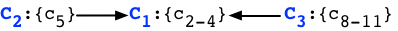
\includegraphics[scale=0.6]{DepDAG.png}
\end{figure}
\vspace*{-0.08in}
Each node (labeled $C_i$) is a set of constraints that belong to a
strongly connected component in the dependency graph ($G_c$), hence
are mutually dependent. All dependencies, except the self-dependency
on $\mathbf{c_{10}}$, are type-2 dependencies.

A dependency DAG makes the dependencies between constraints explicit.
Constraints in each set are mutually dependent, and need to be solved
simultaneously, whereas constraints in different sets can be solved as
per any valid topological ordering of the graph's transpose.
Accordingly, we obtain a topological ordering of nodes in the graph
$G_{{C}}^{T}$ ($G_C$'s transpose), and solve the sets of constraints
in that order. The solutions obtained after solving a constraint set
are applied to the constraints in subsequent sets before attempting to
solve them. For the DAG in figure above, we consider the topological
order $[C_1, C_2, C_3]$ of its transpose, and solve the sets of
constraints in that order.

% Consequently, when the turn of a constraint set ($C$) arrives during
% the constraint solving process, it satisfies certain properties:
% \begin{itemize}
% \item There exists only one predicate variable ($\varphi$) that is either
% constrained or used by the constraints in the set ($C$). The variable is
% called set's \emph{subject}. This property follows from (a). the fact
% that all the dependency constraints have already been solved (and
% solutions applied), and (b). the assumption that there are no mutually
% recursive definitions. 
% \item All the constraints that constrain the set's subject are present
% in the set. This follows from our definition of the dependency relation.
% \end{itemize}

Solving a set ($C$) of constraints involves finding assignments for
free region ($\rho$) and predicate ($\varphi$) variables in the set.
Assignments to region variables can be found via unification (for the
examples in \S~\ref{sec:constraints}, we have already performed the
unification, so $C_{1-3}$ do not contain free region variables). Once
the region variables have been unified, we solve $C$ to find an
assignment for free predicate variables. The first step is to reduce
the set of constraints into an equivalent single constraint by
conjoining antecedents and consequents of all constraints in the
set\footnote{Supplement contains formal justification for this step}.
For the constraint sets $C_1$, $C_2$, and $C_3$, the equivalent
constraint are $c_{12}$, $c_{13}$, and $c_{14}$, respectively, shown
below:
\begin{smathpar}
\begin{array}{l}
  \csid{12} \isvalid{\varphi_0}{\rho_0 \outlives \rhoalloc_0 \conj \rho_1
     \succeq \rhoalloc_0 \conj \rho_4 = \rhoalloc_0 \conj 
     \rho_2 = \rho_0 \conj \rho_3 = \rho_1}\\
  \csid{13} \isvalid{\varphi_0 \conj \varphi_1} {\rho_5 = \rho_0}\\
  \csid{14} \isvalid{\varphi_1 \conj \varphi_2 \conj \rgn_0 \outlives \rgn_1} 
    {
        \rho_7 \outlives \rho_6 \conj \rho_8 \outlives \rho_6 \conj 
        \rho_7 = \rho_9 \conj 
    }\\
  \hspace*{1.4in} \rho_{8} = \rho_9 \conj
        [\rgn_1/\rhoalloc_2][\rgn_1/\rho_6][\rgn_0/\rho_{7-9}]\varphi_2
\end{array}
\end{smathpar}
The constraint $c_{12}$ is a non-recursive constraint of the form
$\isvalid{\phictxt \conj \varphi}{\phicstr}$, where $\phictxt$ and
$\phicstr$ are concrete constraint formulas ($\phictxt$ is $true$ in
this case). Note that the constraint describes an abduction problem,
whose solution is the weakest $\phisol$ such that $\isvalid{\phictxt
\conj \phisol}{\phicstr}$. We solve the problem by casting it as an
instance of graph augmentation problem~\cite{siam92}. Our intuition is
based on the observation that a constraint can be viewed as a directed
graph with region variables as vertices and outlives relationships
between them as edges (equality is encoded as a conjunction of
symmetric outlives relationships).  Let $G(\phictxt)$ and
$G(\phicstr)$ represent such graphs for $\phictxt$ and $\phicstr$,
respectively. Now, $\isvalid{\phictxt}{\phicstr}$ if and only if every
pair $(\rho_1,\rho_2)$ of connected vertices in $G(\phicstr)$ are also
connected in $G(\phictxt)$. If $\rho_1$ and $\rho_2$ are not connected
in $G(\phictxt)$, then it means that $\isvalid{\phicstr}{\rho_1
\outlives \rho_2}$ but $\isnotvalid{\phictxt}{\rho_1 \outlives
\rho_2}$. Since $\phisol$ needs to satisfy $\isvalid{\phictxt \conj
\phisol}{\phicstr}$, it must be the case that $\rho_1$ and $\rho_2$
are connected in $G(\phictxt) \cup G(\phisol)$. Since $\phisol$ must
be weakest such formula, it can be obtained by computing the minimum
number of edges that need to be added to $G(\phictxt)$ such that it is
``as connected as'' $G(\phicstr)$. Using this technique, we obtain the
following solutions to $\varphi_0$ and $\varphi_1$ for constraints in
the running example:
\begin{center}
\(
  \varphi_0 \Leftrightarrow \rho_0 \outlives \rhoalloc_0 \conj \rho_1
     \succeq \rhoalloc_0 \conj \rho_4 = \rhoalloc_0 \conj 
     \rho_2 = \rho_0 \conj \rho_3 = \rho_1
\)\\
\(
  \varphi_1 \Leftrightarrow \rho_5 = \rho_0
\)
\end{center}
Substituting the above solutions for $\varphi_0$ and $\varphi_1$ in
$c_{14}$ gives us a recursive constraint of the following form:
\begin{center}
\(
  \isvalid{\phictxt \conj \varphi}{\phicstr \conj F(\varphi)}
\)
\end{center}
Where $\phictxt$ and $\phicstr$ are concrete constraint formulas, and $F$ is
a substitution function, not necessarily idempotent. Our solution to the
constraints of the above form is based on the observation that $H(\varphi) =
\phicstr \conj F(\varphi)$ is a monotone over the complete meet semi-lattice
of all possible constraints over the domain of region variables in the
program. Hence, by Tarski's fixpoint theorem~\cite{tarski}, $H$ has a
greatest fixed point. To solve the recursive constraint, we first compute the
greatest fixed point ($\phi_f$) for $H$, and then solve the non-recursive
constraint $\isvalid{\phictxt \conj \varphi}{\phi_f}$ using the graph
approach described above. Using this approach, we solve the recursive
constraint $c_{14}$, to obtain the following solution to $\varphi_2$:
\begin{center}
\(
  \rho_7 \outlives \rho_6 \conj \rho_8 \outlives \rho_6 \conj \rho_7 =
  \rho_9 \conj \rho_8 = \rho_9
\)
\end{center}

% If such $\phisol$ satisfies the
% well-formedness condition on $\varphi$, then it is clearly a solution
% for $\varphi$, because there cannot exist a weaker solution for
% $\varphi$ that implies $\phicstr$ under $\phictxt$. On contrary, if a
% maximally weak $\phisol$ fails the well-formedness condition, then we
% establish~\cite{techrep} that it is impossible to satisfy the
% constraint. Hence, it suffices to obtain a maximally weak $\phisol$,
% that satisfies $\isvalid{\phictxt}{\phisol \Leftrightarrow \phicstr}$
% and check if it satisfies the well-formedness condition on $\varphi$.

% \vspace*{-0.05in}
% \paragraph{Definitions} Given a constraint formula $\phi$, we define
% its graph encoding $G(\phi)=(V(\phi),E(\phi))$ as a digraph whose
% vertices ($V(\phi)$) are free region variables and identifiers in
% $\phi$, and whose edges ($E(\phi)$) denote outlives constraints
% in\footnote{We alternate between viewing a constraint formula ($\phi$)
% as a set of constraints and a conjunction of constraints in this
% description} $\phi$.  That is, if $\phi$ contains a constraint $\rho_1
% \outlives \rho_2$, then $\rho_1,\rho_2 \in V(\phi)$ and
% $(\rho_1,\rho_2) \in E(\phi)$. Equality constraints are treated as a
% conjunction of symmetric outlives constraints for the purpose of graph
% encoding. Conversely, given a digraph $G$, we define its constraint
% encoding $\Phi(G)$ in a straightforward manner. We say that a graph
% $G_1=(V_1,E_1)$ is as connected as graph $G_2=(V_2,E_2)$ if $V_2
% \subseteq V_1$, and for every $\rho_1, \rho_2 \in V_2$, if there
% exists a path between $\rho_1$ and $\rho_2$ in $G_2$, then there must
% exist a path between same pair of vertices in $G_1$. 

% A maximally weak $\phisol$ that satisfies $\isvalid{\phictxt}{\phisol
% \Leftrightarrow \phicstr}$ is a constraint encoding of the smallest
% graph $G$ (i.e., $\Phi(G)$) such that $G(\phictxt) \cup G$ is as
% connected as $G(\phicstr)$. The problem of computing such a $G$ is
% equivalent to the problem finding of finding minimum number of edges
% to add to $G(\phictxt)$ such that it is as connected as $G(\phicstr)$.
% Efficient algorithms to solve the later problem are known to
% exist~\cite{graph}, and we rely on them for the solution.

% Solving the constraints $c_{12}$ and $c_{13}$ by reducing them to
% graph augmentation problems, as described above, results in the
% following solutions for $\varphi_0$ and $\varphi_1$ (symmetric
% outlives constraints are replaced with equalities):
% \begin{center}
% \(
%   \varphi_1 \Leftrightarrow \rho_0 \outlives \rhoalloc_0 \conj \rho_1
%      \succeq \rhoalloc_0 \conj \rho_4 = \rhoalloc_0 \conj 
%      \rho_2 = \rho_0 \conj \rho_3 = \rho_1
% \)\\
% \(
%   \varphi_2 \Leftrightarrow \rho_5 = \rho_0
% \)
% \end{center}
% Substituting the above solutions for $\varphi_0$ and $\varphi_1$ in
% $c_{14}$ gives us a recursive constraint of the following form:
% \begin{center}
% \(
%   \isvalid{\phictxt \conj \varphi}{\phicstr \conj F(\varphi)}
% \)
% \end{center}
% Where $\phictxt$ and $\phicstr$ are concrete constraint formulas, and
% $F$ is a substitution function, not necessarily idempotent. Let
% $G(\varphi) = \phicstr \conj F(\varphi)$, so that the constraint is
% $\isvalid{\phictxt \conj \varphi}{H(\varphi)}$. Our solution to such
% recursive constraints  is based on some observations. Firstly, the set
% of all possible constraints over a finite set of region
% variables/identifiers is a complete meet semi-lattice, where (a).
% meet operation is defined as $\phi_1 \sqcap \phi_2 \triangleq \phi_1
% \conj \phi_2$, and (b). lattice order is defined as $\phi_1 \le \phi_2
% \triangleq \isvalid{\cdot}{\phi_1 \Rightarrow \phi_2}$. Secondly,
% function $H$ is a monotone over the lattice since $\forall
% \phi_1,\phi_2.\; \isvalid{\cdot}{(\phi_1 \Rightarrow \phi_2)
% \Rightarrow (H(\phi_1) \Rightarrow H(\phi_2))}$. From Knaster-Tarski's
% theorem, we know that $H$ has a greatest fixed point $\phi_f$ such
% that $\isvalid{\cdot}{\phi_f \Leftrightarrow H(\phi_f) }$. To solve
% the recursive constraint shown above, we first compute the greatest
% fixed point ($\phi_f$) of $H$, and then reduce the constraint to the
% following non-recursive constraint:
% \begin{center}
% \(
%   \isvalid{\phictxt \conj \varphi}{\phi_f}
% \)
% \end{center}
% Which can then be solved via the graph-based approach described
% before.

% Let $H(\varphi_2)$ denote the consequent of the recursive constraint
% $c_{14}$. Its greatest fixed point ($\phi_f$) is shown below:
% \begin{center}
% \(
%   \rho_7 \outlives \rho_6 \conj \rho_8 \outlives \rho_6 \conj \rho_7 =
%   \rho_9 \conj \rho_8 = \rho_9 \conj \rgn_0 \outlives \rgn_1 \conj
%   \rgn_0 = \rgn_0
% \)
% \end{center}
% Computing a maximally weak $\phisol$ such that $\isvalid{\varphi_1
% \conj \rgn_0 \outlives \rgn_1}{\phisol \Leftrightarrow \phi_f}$
% results in the following solution for $\varphi_2$ that meets its
% well-formedness requirement ($\tywf{\{\rhoalloc_0,\rho_{}0-4,
% \rhoalloc_2, \rho_{6-9}\}}{\varphi_2} $):
% \begin{center}
% \(
%   \rho_7 \outlives \rho_6 \conj \rho_8 \outlives \rho_6 \conj \rho_7 =
%   \rho_9 \conj \rho_8 = \rho_9
% \)
% \end{center}

\subsection{Higher-Order Type Inference}

% The region type system for $\FB$ admits function types with
% higher-rank region polymorphism, allowing region variables to be
% quantified in the types of higher-order arguments. This allows, for
% example, a user-defined function to be applied on arguments from
% different regions in different contexts. However, like most type
% systems, our region type system loses principal typing property in
% presence of higher-rank polymorphism, which means that there can be
% two possible types for a function, where neither one is more general
% than the other. Consequently, it is not possible to infer a unique
% type for a function. Nonetheless, it is possible to engineer type
% inference to to consistently prefer one type over the other.
Our type inference algorithm does not straightforwardly generalize to
the higher-order case, due to the lack of principal typing in presence of
higher-rank polymorphism. Fortunately, higher-order type inference, in
its full generality, is rarely needed in the context of \name, where
higher-order control flow is predominantly due to the second-order
arguments to constructors (For \eg, user-defined functions in dataflow
queries, and lambda arguments to the $\RgnZ$ class constructor). We
therefore extend our inference algorithm with a heuristics tailor-made
for the aforementioned second-order cases. The simplistic approach
seems to suffice in our experience, but, it is always possible that it
makes the type checker reject a program that is otherwise valid. In
such cases, programmer can help the type checker by writing region
annotations only over higher-order arguments.  Nonetheless, we note
that it is possible to infer most general (if not principal) types for
higher-order arguments, by extending our constraint solver with an
approach modeled after~\cite{gulwani09}, which lets it compute maximally
weak/strong solutions to multiple competing $\varphi$'s
simultaneously.

% \begin{codejava}
% bool app2(A x, A y, (A $\rightarrow$ bool) f) 
%     { return (f x && f y); }
% \end{codejava}
% There are two possibilities for the region type of \C{app2}: one,
% where it allows \C{x} and \C{y} to be allocated in different regions,
% but requires \C{f} to be region-polymorphic (i.e, \C{f} should accept
% arguments from any region), and second, where it requires \C{x} and
% \C{y} to be allocated in the same region, and allows \C{f} to be
% monomorphic. None of the two types are more general than the other,
% and it is not clear which one is more preferable. The concrete
% manifestation of this dilemma is a constraint of form 
% $\isvalid{\phictxt \conj \varphi_1}{\phicstr \conj \varphi_2}$, with
% no additional constraints to help determine $\varphi_1$ or $\varphi_2$
% before solving this constraint. Since it is always possible to
% strengthen $\varphi_2$ and then find a suitable $\varphi_1$, there
% does not exist unique solution to such constraints. Nonetheless, it is
% possible to bias the constraint-solving algorithm to consistently
% prefer one solution over the other.

% In context of \name, however, we adopt a trivial solution of
% assigning the same region to the arguments and return values in
% (higher-order) function types. For user-defined functions (e.g.,
% predicate in the \C{WHERE} clause of the \C{SELECT} dataflow query)
% and lambda arguments to the $\RgnZ$ class constructor, which are the
% prominent uses of higher-order functions in \name, the simplistic
% approach seems to suffice in practice. However, it is always possible
% that this approach makes type checker reject a program that is
% otherwise valid. In such cases, programmer can help the type checker
% by writing region annotations for only the higher-order functions.

% \begin{center}
%   \C{app2} : $\inang{\rho_0,\rho_1}$(\C{A}$\inang{\rho_0}$, 
%               \C{A}$\inang{\rho_0}$,
%               $\inang{\rho_2}$\C{A}$\inang{\rho_2}$ $\rightarrow$
%               \C{bool}) $\rightarrow$ \C{bool}
% \end{center}
